\chapter{Aandrijving}
De combinatie van het uitlezen van sensoren met het aandrijven van hardware vormt de basis van alle meet- en regel systemen. Dit hoofdstuk bevat recepten voor het aansturen van hardware.

\section{Transistors}
\paragraph{Probleem:}
Je wilt een systeem aansturen dat meer power nodig heeft dan je I/O pinnen kunnen leveren, zie hoofdstuk~\ref{sec:VeiligOmgaan}. Door middel van een transistor kan het circuit, net als met een schakelaar, open en gesloten worden. Een I/O pin stuurt deze 'schakelaar' aan, terwijl een externe bron de stroom levert.

\paragraph{Benodigdheden:}
\begin{itemize}
	\item 1x LED
	\item 1x \SI{100}{\ohm} weerstand
	\item 1x \SI{3.9}{\kilo\ohm} weerstand
	\item 1x NPN transistor (BJT)
\end{itemize}

\paragraph{Oplossing}: 

	\begin{figure}
		\center{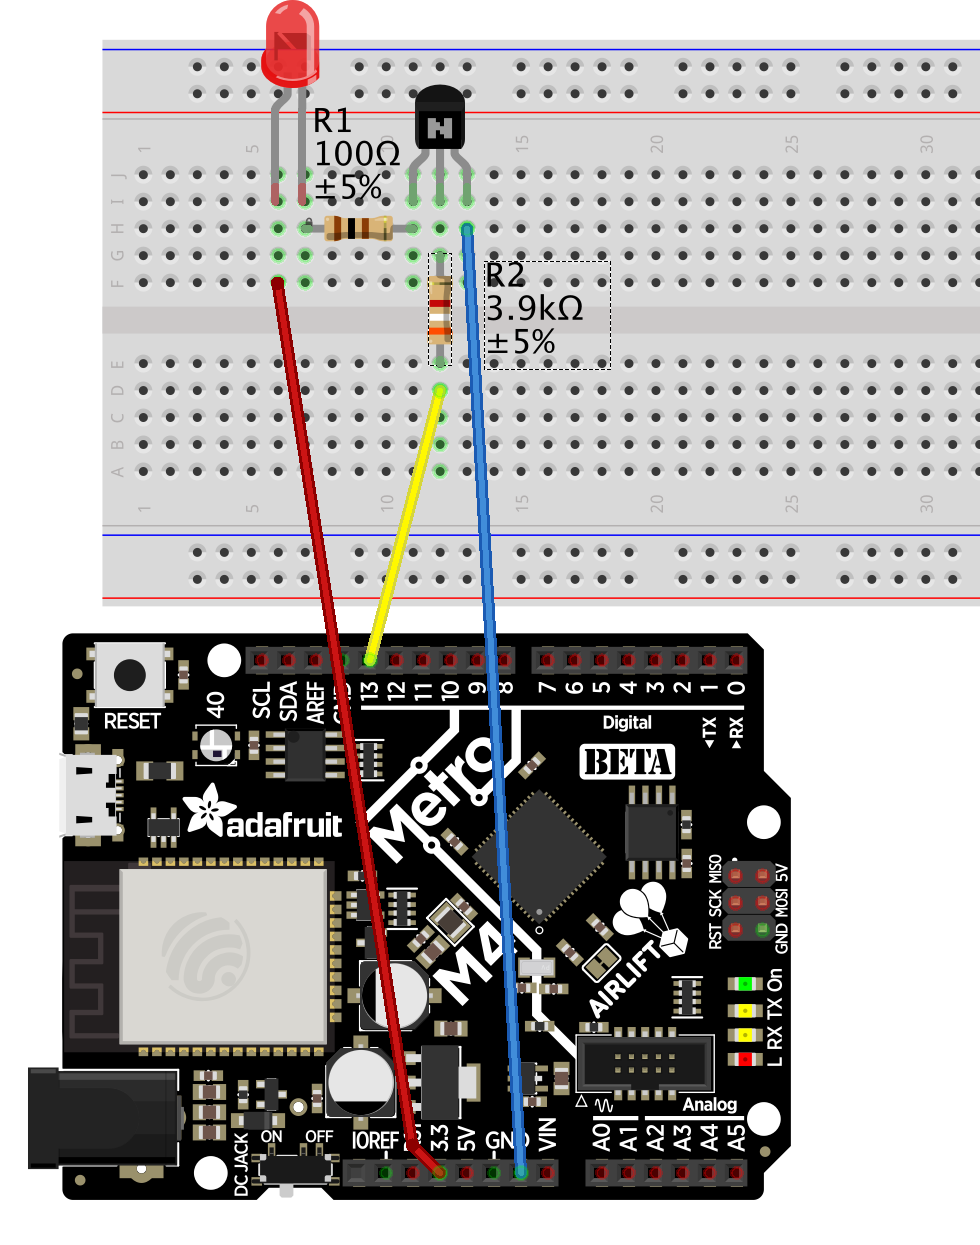
\includegraphics[width=0.5\linewidth]{figures/TransistorLED.png}}
		\caption{Transistor Circuit}
		\label{fig:TransistorLED}
	\end{figure}

\paragraph{Transistor Berekening:}
\begin{figure}
	\center{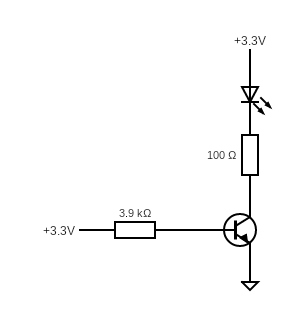
\includegraphics[width=0.6\linewidth]{figures/Transistorcircuit.png}}
	\caption{Transistor Diagram}
	\label{fig:TransistorDiagram}
\end{figure}

\begin{alignat}{9}
\beta &\approx 25\to 100\\
V_{source}&=\SI{3.3}{\volt}\\
V_{CE}&=\SI{0.1}{\volt}\\
V_{BE}&=\SI{0.8}{\volt}\\
V_{LED}&=\SI{2}{\volt}\\
I_{C_{Verzadigd}}&=\SI{12}{\milli\ampere}\\
I_B&>\frac{I_{C_{SAT}}}{25}=\SI{0.48}{\milli\ampere}\\
R_C& \approx \frac{V_{source}-V_{CE}-V_{LED}}{I_{C_{SAT}}} \approx \SI{100}{\ohm}\\
R_B& < \frac{V_{source}-V_{BE}}{I_B}<\SI{5.2}{\kilo\ohm}
\end{alignat}

\paragraph{Discussie:} Transistors zijn op verschillende manieren te gebruiken. Als versterker of als schakelaar. In dit voorbeeld wordt de transistor als schakelaar gebruikt. Eerst moet bepaald worden hoeveel stroom er door de LED moet. Maximale stroom door een LED is vaak rond de \SI{20}{\milli\ampere}. In dit voorbeeld wordt een veilige stroom van \SI{12}{\milli\ampere} genomen. Op basis van de Collector-Emitter spanningsval(te vinden in de transistor datasheet), de spanningsval over de LED en de bronspanning kan de weerstand in serie met de LED berekend worden. Met deze weerstand is de \SI{12}{\milli\ampere} de maximale stroom die van de collector naar de emitter kan stromen. Dit is dan ook de stroom die loopt als de transistor verzadigd is. Om de transistor als schakelaar te gebruiken en niet als versterker, moet er voor gezorgd worden dat de Base-Emitter stroom hoog genoeg is om de transistor te verzadigen. Dit is afhankelijk van de verzadigde stroom(\SI{12}{\milli\ampere}) en de \textit{gain} of versterking $\beta$. $\beta$ is te vinden in de data sheet en ligt vaak tussen de 25 en 100. Om er zeker van te zijn dat verzadiging bereikt wordt, wordt met een lage versterking van 25 de benodigde base-emitter stroom bepaald. De benodigde base-emitter stroom kan vervolgens samen met de bronspanning en base-emitter spanningsval gebruikt worden om de weerstand aan de base te berekenen.

\newpage



\section{DC Motor}\label{sec:DCMotor}
\paragraph{Probleem:}
Je wilt een DC aansturen met je micro-controller, dat zowel vooruit als achteruit kan draaien.

\paragraph{Benodigdheden:}
\begin{itemize}
	\item 1x 9V batterij
	\item 1x L298N H-Bridge Motor Driver
	\item 1x DC Motor
\end{itemize}

\paragraph{Oplossing}:

	\begin{figure}[H]
		\center{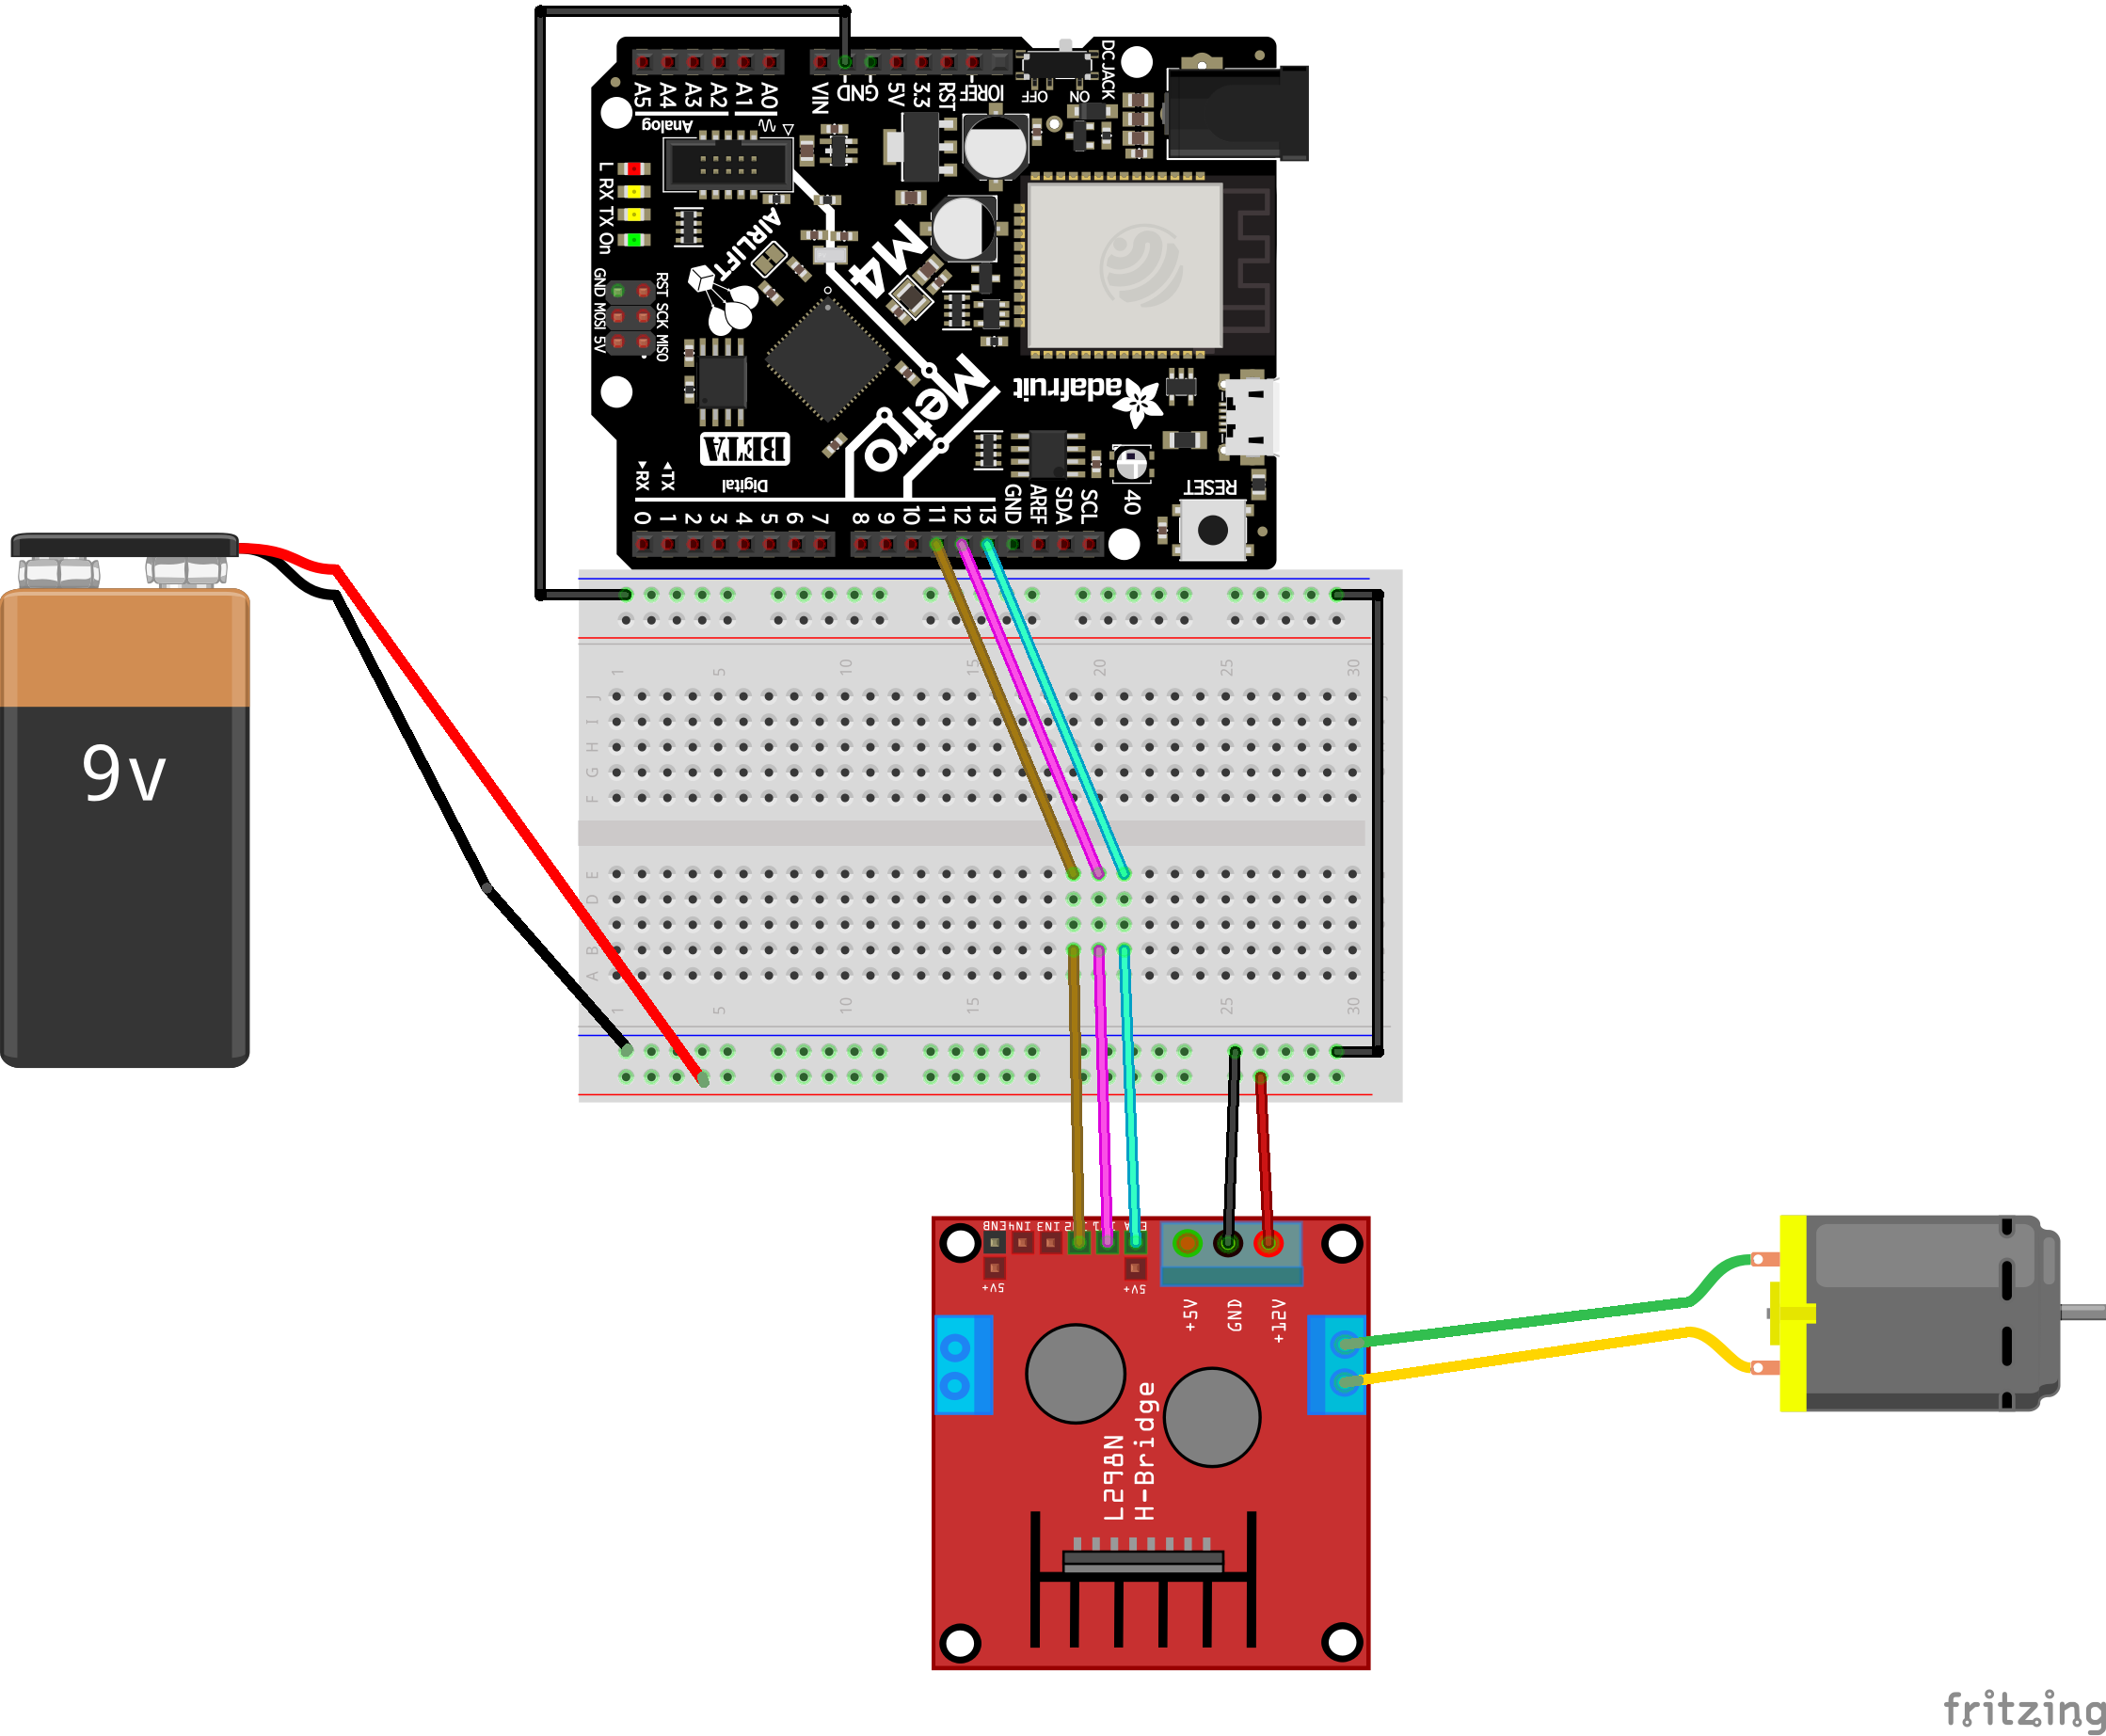
\includegraphics[width=\linewidth]{figures/DC_Motor.png}}
		\caption{MotorDriver Circuit}
		\label{fig:MotorDriver}
	\end{figure}
\newpage
		\lstinputlisting{code/DC_Motor.py}

	

\paragraph{Discussie:} Het bordje kan zelf niet het vermogen leveren voor de motor en met alleen een positieve spanning kan de motor normaal gesproken maar in 1 richting draaien. Met het gebruik van een H-brug kan zowel een externe spanningsbron gebruikt worden als in 2 richtingen gedraaid worden. Met de IN1 en IN2 pinnen op de H-brug kan de richting ingesteld worden door op 1 pin een hoge spanning te zetten en op de ander een lage spanning. Met de ENA pin wordt de motor aan en uit gezet. Door hier een blok golf op te zetten met PWM kan ook de snelheid geregeld worden door de duty cycle aan te passen. 

In de code worden zoals gewoonlijk eerst de benodigde modules geimporteerd. Daarna wordt gedefinieerd welke I/O pinnen zijn aangesloten op de pinnen van de H-brug. De ENA pin wordt geinitaliseerd als PWM, en de IN1 en IN2 als digitale outputs. Er worden ook functies gedefinieerd om de motor vooruit en achteruit te laten draaien, met als input de duty cycle. Allebei de functies werken hetzelfde. Eerst wordt de motor uitgezet, dan wordt de richting bepaald door de IN1 en IN2 pinnen en dan wordt de motor aan gezet met de juiste duty cycle.

De oneindige while loop laat de motor een halve seconde vooruit draaien en daarna een halve seconde achteruit.



\section{Twee DC motoren}\label{sec:TwoDCMotors}
	\paragraph{Probleem:} Je wilt twee DC motoren tegelijkertijd aansturen.
	
	\paragraph{Benodigdheden:}
	\begin{itemize}
		\item 1x 9V batterij
		\item 1x L298N H-Bridge Motor Driver
		\item 2x DC Motor
	\end{itemize}
	
	\paragraph{Oplossing}: 
	\lstinputlisting{code/Two_DC_Motor.py}
	
	\begin{figure}[H]
		\center{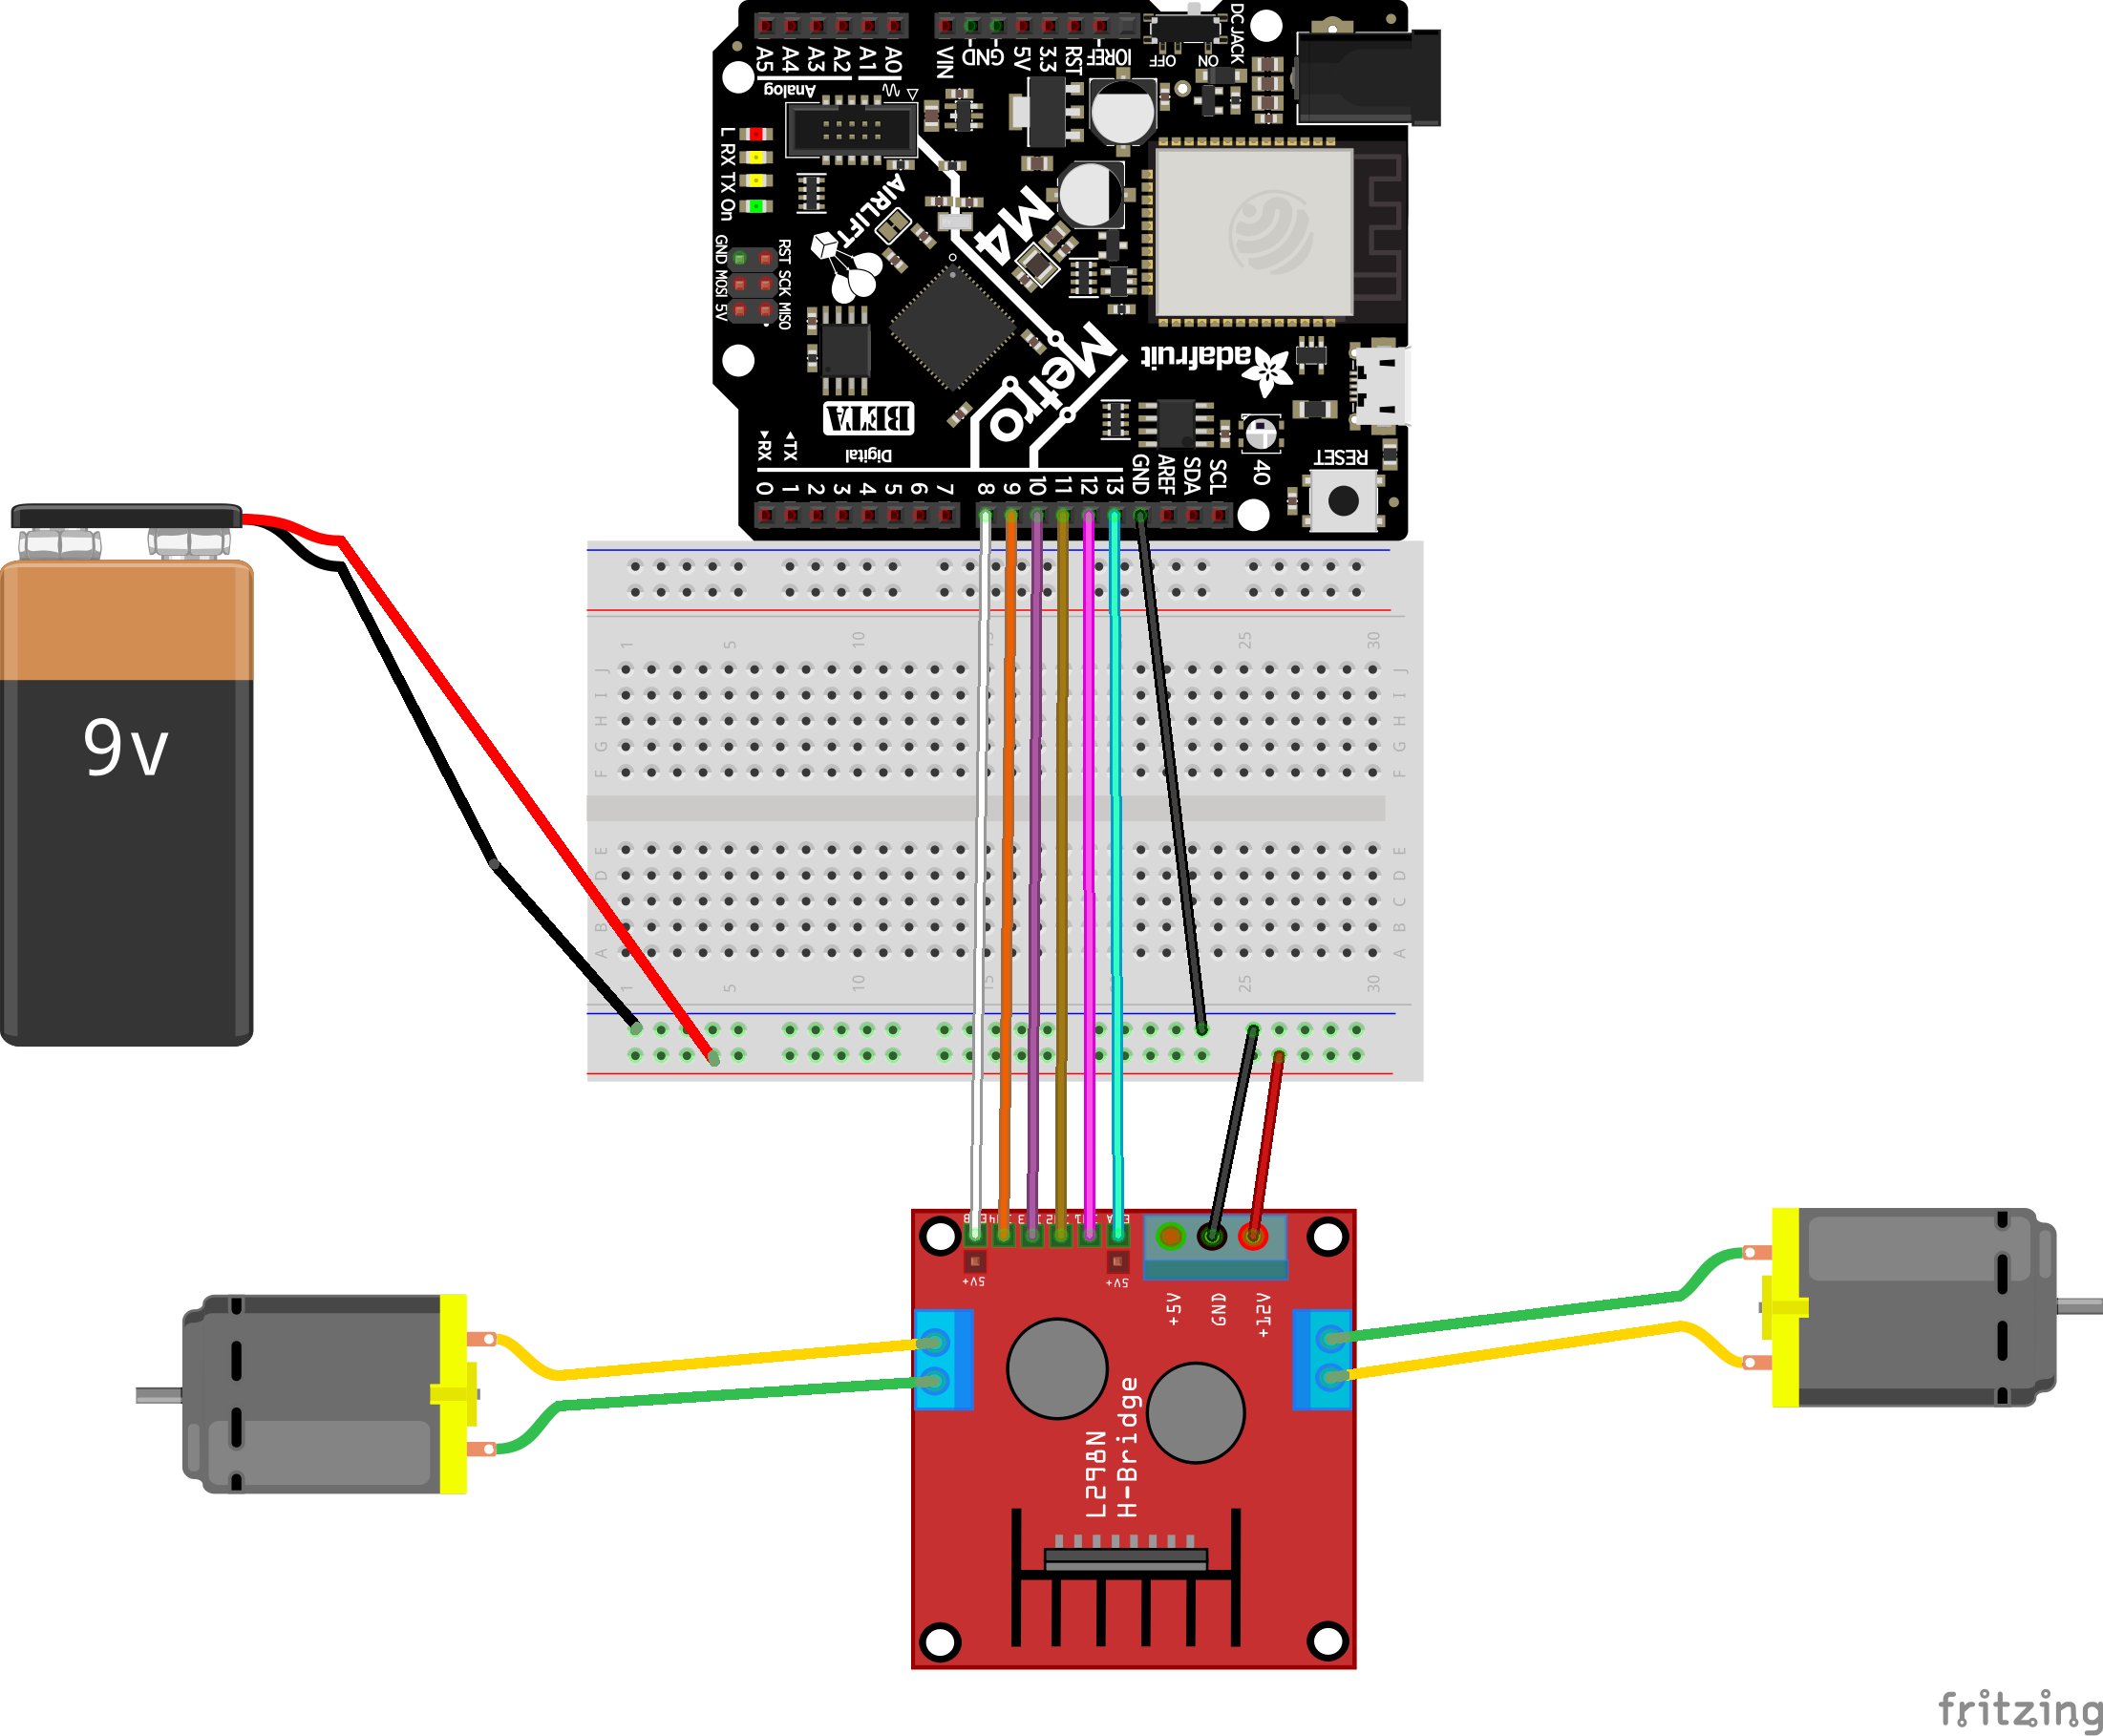
\includegraphics[width=0.8\linewidth]{figures/MotorDriver.png}}
		\caption{Double Motor Driver Circuit}
		\label{fig:Two_DC_Motor}
	\end{figure}

	\paragraph{Discussie:} De code is haast hetzelfde als met 1 DC motor in recept~\ref{sec:DCMotor}, maar alles dubbel gedefinieerd. 
	
\newpage
\section{Servo}\label{sec:servo}
\paragraph{Probleem:} Je wilt een Servo aansturen.

\paragraph{Benodigdheden:}
\begin{itemize}
	\item 1x Servo
\end{itemize}

\paragraph{Oplossing}:

\begin{figure}[H]
	\center{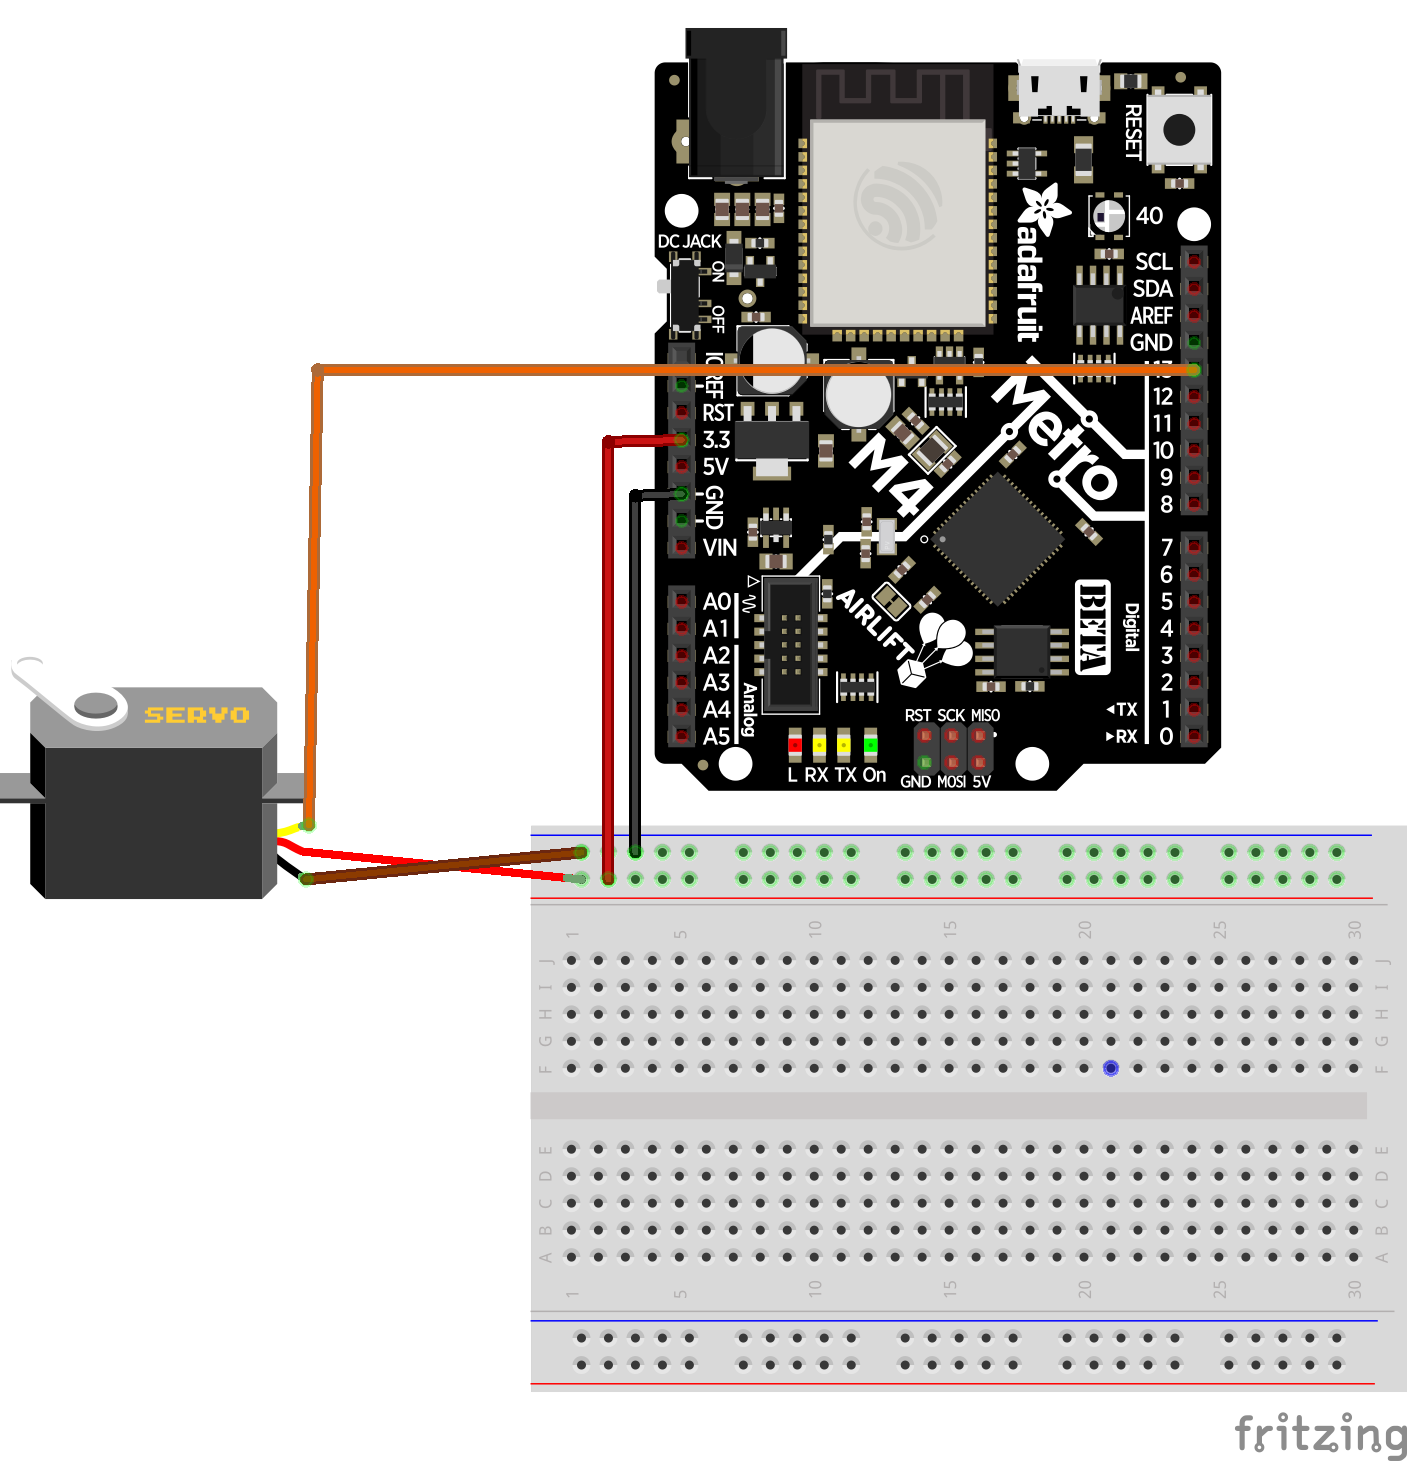
\includegraphics[width=0.6\linewidth]{figures/Servo.png}}
	\caption{Servo Circuit}
	\label{fig:Servo}
\end{figure}

\newpage
\lstinputlisting{code/Servo.py}
\paragraph{Discussie:} Voor het aansturen van een servo hoef je zelf weinig te programmeren, want adafruit heeft hier een speciale bibliotheek voor in hun CircuitPython library bundel. Deze bundel kan je vinden op \url{https://circuitpython.org/libraries}. Zorg dat de adafruit\_motor map in de lib folder op je bordje staat. \\

Importeer de servo module van de adafruit\_motor bibliotheek en ook de time, board en pulsio modules. Een servo object kan eenvoudig gemaakt worden door een pwm object aan de Servo() functie van de servo module te geven. Daarna kan de hoek van de servo ingesteld worden door objectnaam.angle van het servo object aan te passen. In de code gaat de servo van 0 tot 180 graden en terug.\\


\newpage
\section{Twee DC motoren, een servo en een toeter aansturen met een Joystick} \label{sec:DC_Servo_Toeter_Joystick}
\paragraph{Probleem:} Je wilt twee DC motoren tegelijk besturen afhankelijk van hoe ver de joystick naar voren staat. Je wilt tegelijkertijd een servo besturen afhankelijk van hoe ver de joystick naar links en naar rechts staat. Tot slot wil je de toeter aanzetten als je op de joystick drukt.

\paragraph{Benodigdheden:}
\begin{itemize}
	\item 1x 9V batterij
	\item 1x L298N H-Bridge Motor Driver
	\item 2x DC Motor
	\item 1x Servo
	\item 1x \SI{100}{\ohm} weerstand
	\item 1x \SI{8}{\ohm} Speaker
\end{itemize}

\paragraph{Oplossing}:
\begin{figure}[H]
	\center{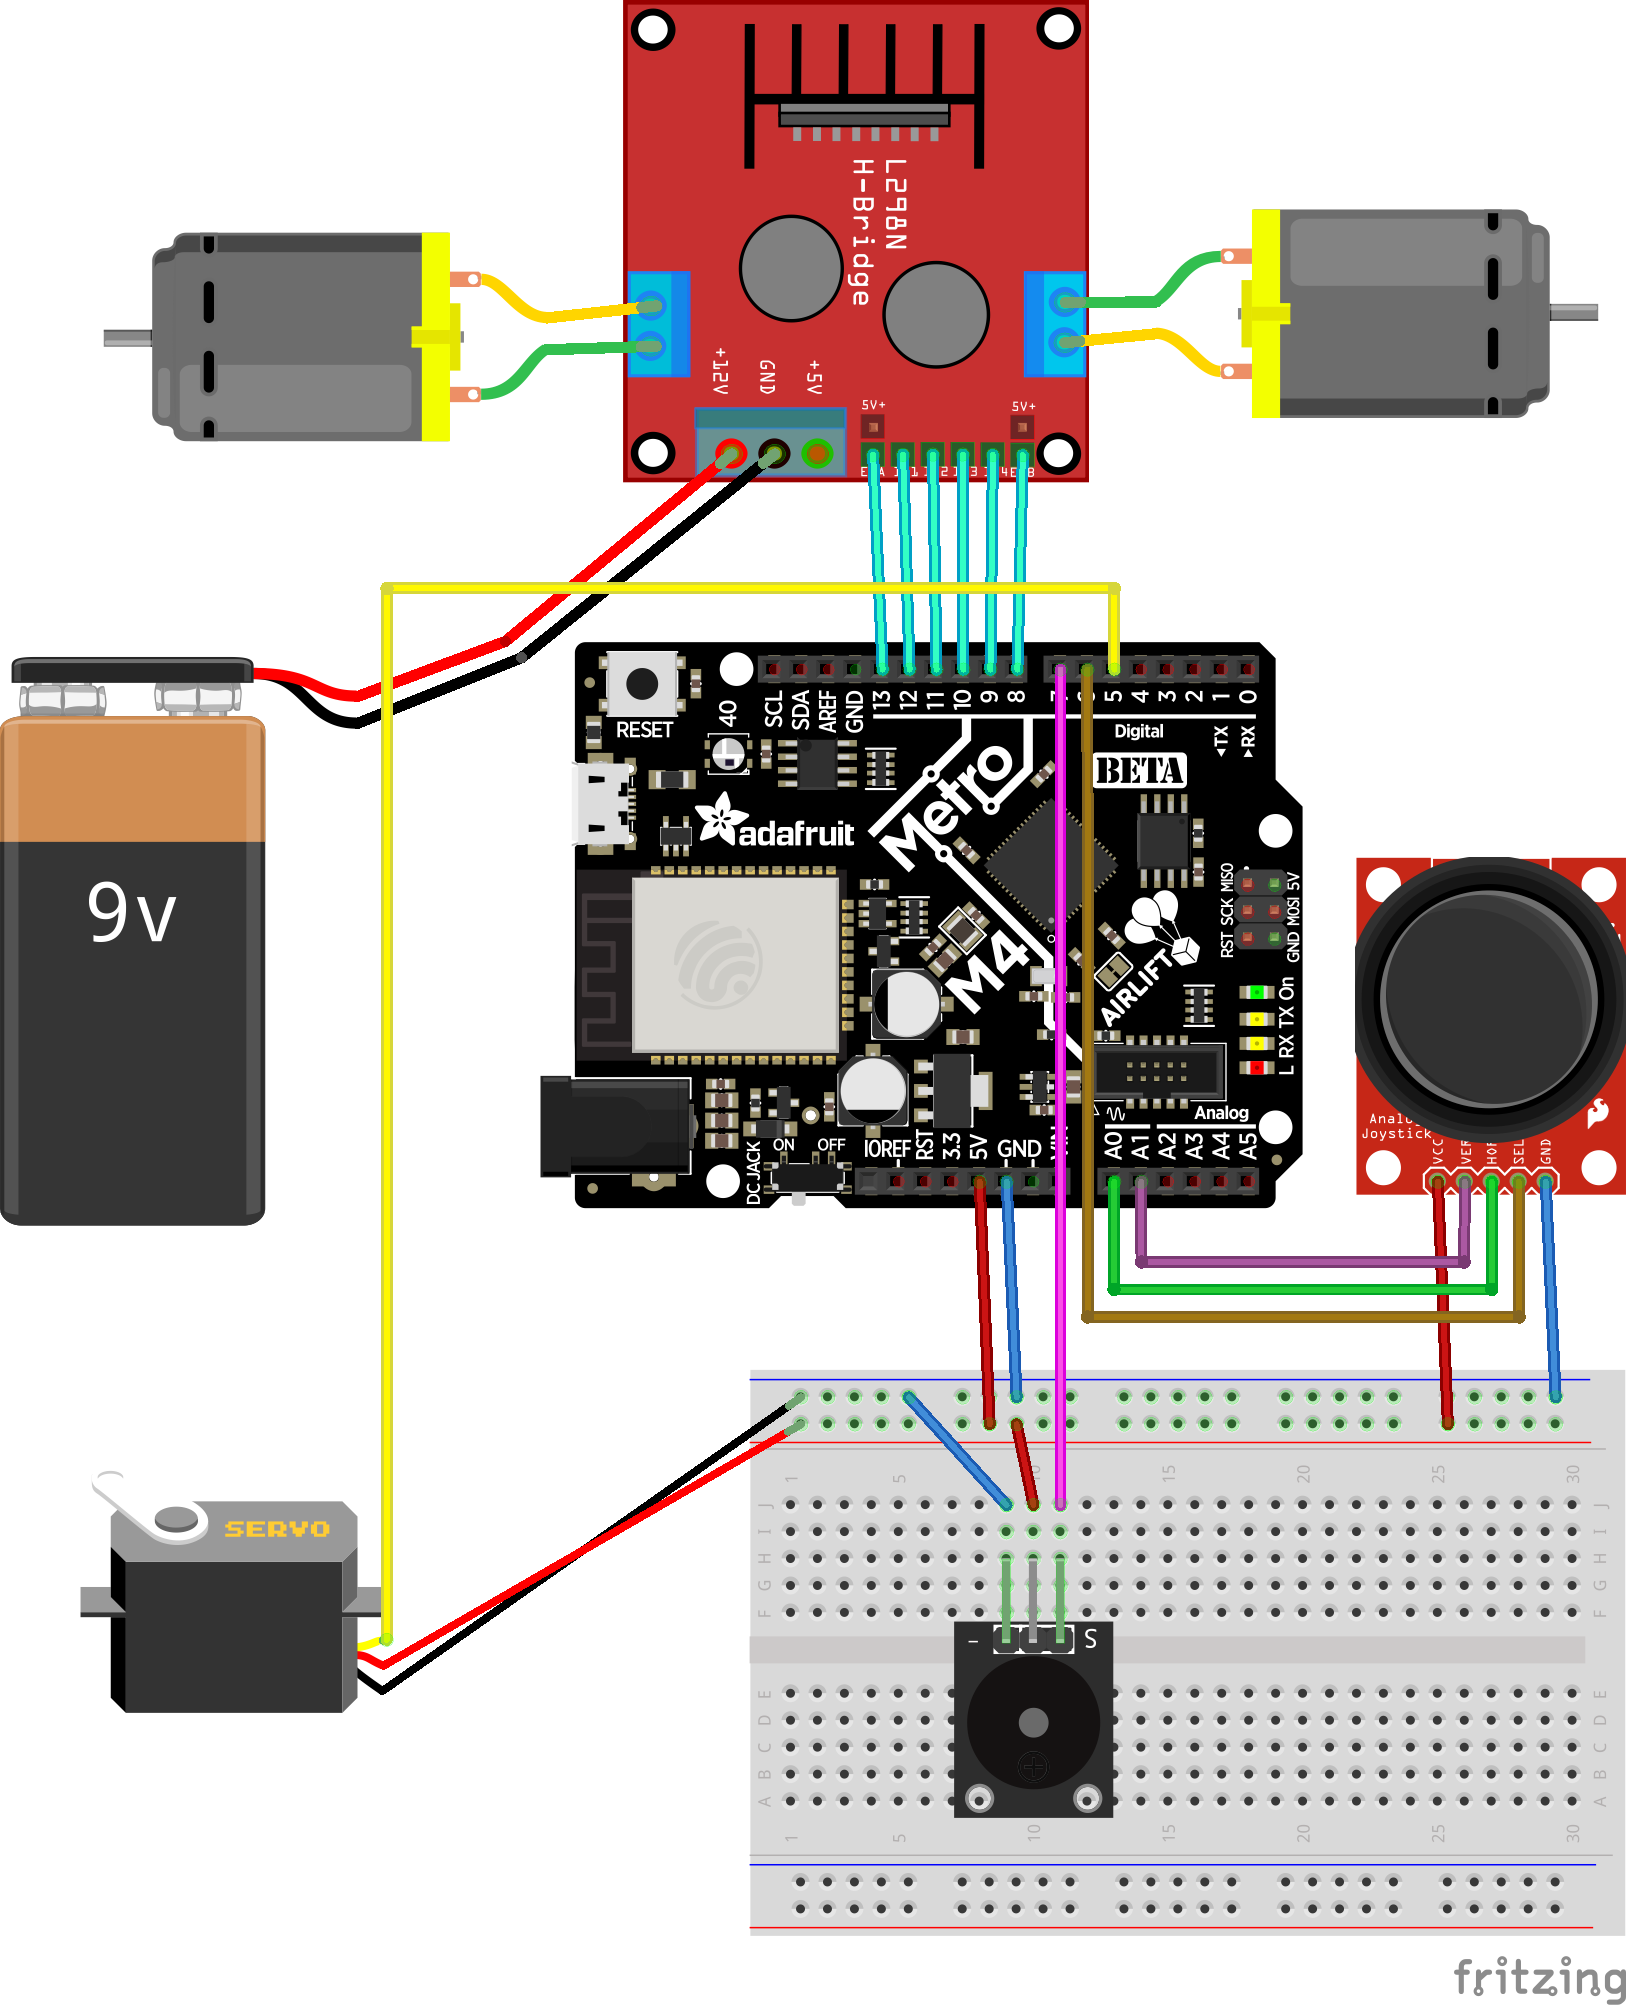
\includegraphics[width=0.7\linewidth]{figures/DC_Servo_Toeter_Joystick.png}}
	\caption{Twee DC motoren, een servo en een toeter aangestuurd door een joystick circuit}
	\label{fig:DC_Servo_Toeter_Joystick}
\end{figure}

\lstinputlisting{code/Two_DC_Motors_Servo_Joystick.py}

\newpage
\paragraph{Discussie:}	Naarmate code meer gaat doen, wordt code vaak ook langer. Het wordt daarom steeds belangrijker om een goede structuur in je code aan te brengen. In deze lap code worden eerst de imports gedaan, daarna de definities, dan de initialisatie en tot slot het programma. 

Vooraf een naam voor de I/O pinnen defini\"eren en later deze naam in de code gebruiken is erg handig. Als je namelijk de ENA pin niet op D13 maar op D2 wilt aansluiten, hoef je alleen de definitie van de ENA\_pin te veranderen en verder niet door de code te zoeken waar je allemaal D13 hebt gebruikt. Ook is het veel makkelijker om te zien of je pinnen per ongeluk dubbel gebruikt.\\

In het kader van het lezen en onderhouden van code kan je zien dat het besturen van een motor in een class is verwerkt. In recept~\ref{sec:TwoDCMotors} moest voor het gebruik van 2 motoren, 2 keer de code voor de initialisatie en voor elke motor een forward() en backward() functie geschreven worden. Als je nog een functie wil schrijven voor het gebruik van de motor, zoals setMotor() in deze code, moet ook dat 2x apart gemaakt worden. Er is een ongeschreven regel in programmeren die zegt 'don't repeat yourself'. Als je jezelf moet herhalen is er vaak een betere manier. 

Het enige verschil tussen de eerste en tweede DC motor is welke pinnen gebruikt worden. De initialisatie en wat er moet gebeuren om de motor voor en achteruit te laten draaien is hetzelfde, alleen moet het dus op andere I/O pinnen gebeuren. Er kan dan een class gemaakt worden voor motoren die de algemene eigenschappen van een motor bij elkaar houdt. Als er een motor is, dan wordt die altijd bestuurd met 3 pinnen. Deze pinnen moeten ge\"initialiseerd worden en worden altijd gebruikt om de snelheid en richting van de motor in te stellen. 

Als dan objectnaam=DC\_Motor() aangeroepen wordt in de code, met als parameters de 3 pinnen, wordt een instantie gemaakt van deze class. Bij het aanmaken van een instantie wordt \textbf{altijd} eerst de \_\_init\_\_ functie doorlopen. Deze initialiseert de pinnen. Elk DC\_Motor object krijgt automatisch zijn eigen forward(), backward() en setMotor() methodes.  Een methode is een functie die hoort bij een class en kan je aanroepen met objectnaam.methode(). De aangemaakte motor1 en motor2 objecten kan je apart aansturen in de code. Je laat motor1 vol vooruit draaien door motor1.forward(1) aan te roepen en motor2 vol achteruit draaien door motor2.backward(1) aan te roepen. Als je een derde motor hebt kan je met 1 regel een extra motor gebruiken.\\

Na de definitie van de class, worden een paar functies gedefinieerd. De "toDutyCycle" functie converteert de uitgelezen 16-bit waarde van de verticale stand van de joystick naar een positieve of negatieve DutyCycle. De "toAngle" functie converteert de horizontale stand naar een hoek en de "setHorn" functie zet de toeter aan als True wordt gegeven als parameter en uit als een False wordt gegeven.\\

Na alle definities worden de motoren, servo, joystick en toeter objecten ge\"initialiseerd. Daarna komt het programma in de oneindige while loop. In deze loop worden de joystick waarden eerst uitgelezen en geconverteerd naar de betekenis van de waarde. JoyStick vol naar achter betekent een duty cycle van -1, vol naar voor +1. Joystick naar links een servo angle van 0 graden, joystick in het midden 90 graden en rechts 180 graden. Knop ingedrukt een waarde True, niet ingedrukt een waarde False. Vervolgens worden deze geconverteerde waarden gebruikt om de motoren, servo en toeter in te stellen.

